%%
%% System Design Analysis
%%

\subsubsection{Rotary Encoder}

\indent\indent For the rotary encoder to be operational and useful, it must be able to determine the angular displacement of the release disks at all times in order to report real-time displacement readings to the RPi for adjusting motor speed via the PID controller in conjunction with the VEX motor speed controller. For this to happen, the MCU in charge of sampling the readings of the IR receiver/emitter pair must have a sampling frequency that it at least 2 times higher than that of the signal generation as per the Nyquist Theorem \cite{Nyq_thm}. Mathematically, the Nyquist Theorem [Eq. ~\ref{eq:Nyq_thm}] is represented as,

\begin{equation}
	f_s \geq 2f_c
    \label{eq:Nyq_thm}
\end{equation}

Where $f_s$ is the sampling frequency in hertz, or how often a signal is sampled per unit time, and $f_c$ is the highest frequency in hertz contained in the signal. The MCU used for the rotary encoder is an ESP32 that runs at 240MHz \cite{espressif}. The ORE pattern found on the release disk was designed to have 54 equally-spaced slits, each pair of slits produces 4 pulses for a total of 216 pulses per revolution (PPR). Taking the highest achievable speed the release disks will experience ($10,000 RPM$ or $166.667 Hz$) and multiplying that by the amount of PPR a frequency of $36kHz$ is achieved.

\begin{equation}
	f_s = 260MHz \geq 2(166.667Hz)(216PPR) = 72kHz = 2f_c
    \label{eq:sampling_rate}
\end{equation}

As seen be seen from [Eq. ~\ref{eq:sampling_rate}], the MCU provides more than enough sampling rate to reliably read and process the signal for use by the RPi.

On the RPi level, the pulse value transmitted by the MCU is then used to compute the displacement and velocity of the tether as follows,

\begin{equation}
	x_{tether} = r_{disk}\times\alpha\times(Pulse)
    \label{eq:tether_dsiplacement}
\end{equation}

\begin{equation}
	\alpha = \sfrac{2\pi}{(54\times4)} = 1.66\degree
    \label{eq:alpha}
\end{equation}

Where $r = 0.1778m$ is the radius of the release disk, $alpha = 1.66$ is the angle resolution as computed in [Eq. ~\ref{eq:alpha}], and $Pulse$ is the pulse value sent by the MCU. From [Eq. ~\ref{eq:tether_dsiplacement}], the displacement value of the tether can be inferred from the ORE readings. In addition to tether displacement, the speed at which the tether is being ejected can also be computed using [Eq. ~\ref{eq:tether_speed}] below,

\begin{equation}
	v_{tether} = \Dot{x}_{tether} = \dfrac{dx_{tether}}{dt}
    \label{eq:tether_speed}
\end{equation}

Where $dx_{tether}$ is the change in the displacement of the tether as computed on the RPi level, and $dt$ is the time span it took for two consecutive pulses to be registered by the MCU as computed on the MCU level. It must be worth noting that floating point operations were kept to a minimum to reduce the computational time needed as to keep the readings as close to real-time as possible.

% ---------------------------------------------------------

\subsubsection{Control Unit}

\indent\indent A RPi was chosen as the controls system's main computing platform. This choice was made due to the RPi's rather small footprint compared to other system on chip (SoC) microcomputers and due to the exceptional community support behind it. In addition to that, the RPi has 40 GPIO readily available for usage by developers alongside 4 USB ports, providing more than adequate connection points for the developers to interface as many peripherals as needed. Furthermore, the RPi has a base clock speed of 1.4GHz, making the RPi a suitable choice for this project.

% ---------------------------------------------------------

\subsubsection{IMU}

\indent\indent Moving on to the sensors, the initial analysis was performed by obtaining the specification sheets for each candidate sensor and the performance parameters were compared, eliminating potential sensors one-by-one until the optimum sensor was picked. Once a sample of the sensors were ordered and received, the sensors were placed under the oscilloscope to monitor the signal being received by the sensors and noise was observed from the power line of the RPi to the sensors at a frequency of $3kH$. To shunt down the noise, the sensors were tested with a combination of capacitors placed as close to the power line as possible and data was collected and recorded for analysis. A sample of the analysis that was done for one of the sensors is found in [Table ~\ref{tab:no_cap} - ~\ref{tab:99nF}] below,

\begin{table}[H]
\caption{\label{tab:no_cap} LSM9DS1 Z-Axis Acceleration Statistics ($C=0F$)}
\centering
\begin{tabular}{l|c}
\hline\hline
\textbf{Statistic}      & \textbf{Value}            \\\hline
Mean                    & $0.99850$                 \\\hline
Median                  & $0.99975$                 \\\hline
Mode  	                & $1.00341$                 \\\hline
Sample Variance         & $2.91\times10^{\minus5}$  \\\hline
Standard Deviation      & $5.39\times10^{\minus3}$  \\\hline
Standard Error  	    & $2.43\times10^{\minus4}$  \\\hline
Minimum                 & $0.98799$                 \\\hline
Maximum                 & $1.00676$                 \\\hline
\end{tabular}
\end{table}

\begin{figure}[ht]
  \centering
  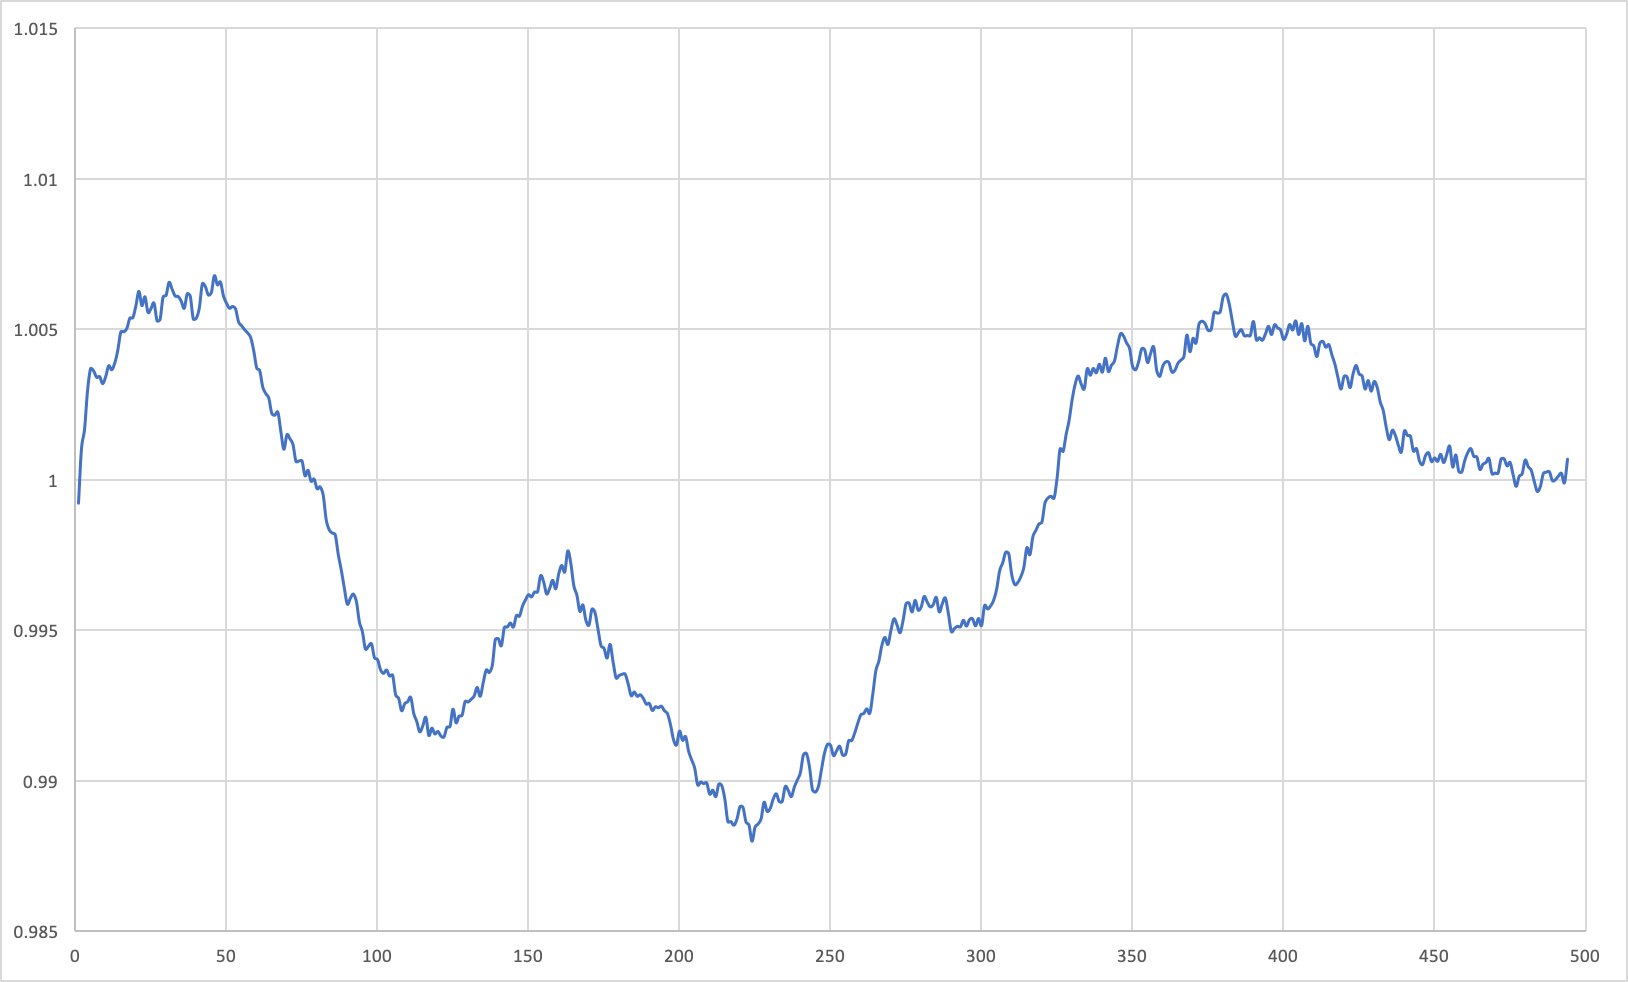
\includegraphics[width=1.0\textwidth]{Controls/no_cap.png}
  \caption{\label{fig:no_cap} LSM9DS1 accelerometer with no capacitor}
\end{figure}

\begin{table}[H]
\caption{\label{tab:10uF} LSM9DS1 Z-Axis Acceleration Statistics ($C=10\mu F$)}
\centering
\begin{tabular}{l|c}
\hline\hline
\textbf{Statistic}      & \textbf{Value}            \\\hline
Mean                    & $1.00095$                 \\\hline
Median                  & $1.00126$                 \\\hline
Mode  	                & $1.00193$                 \\\hline
Sample Variance         & $4.94\times10^{\minus6}$  \\\hline
Standard Deviation      & $2.22\times10^{\minus3}$  \\\hline
Standard Error  	    & $9.97\times10^{\minus5}$  \\\hline
Minimum                 & $0.99373$                 \\\hline
Maximum                 & $1.00502$                 \\\hline
\end{tabular}
\end{table}

\begin{figure}[ht]
  \centering
  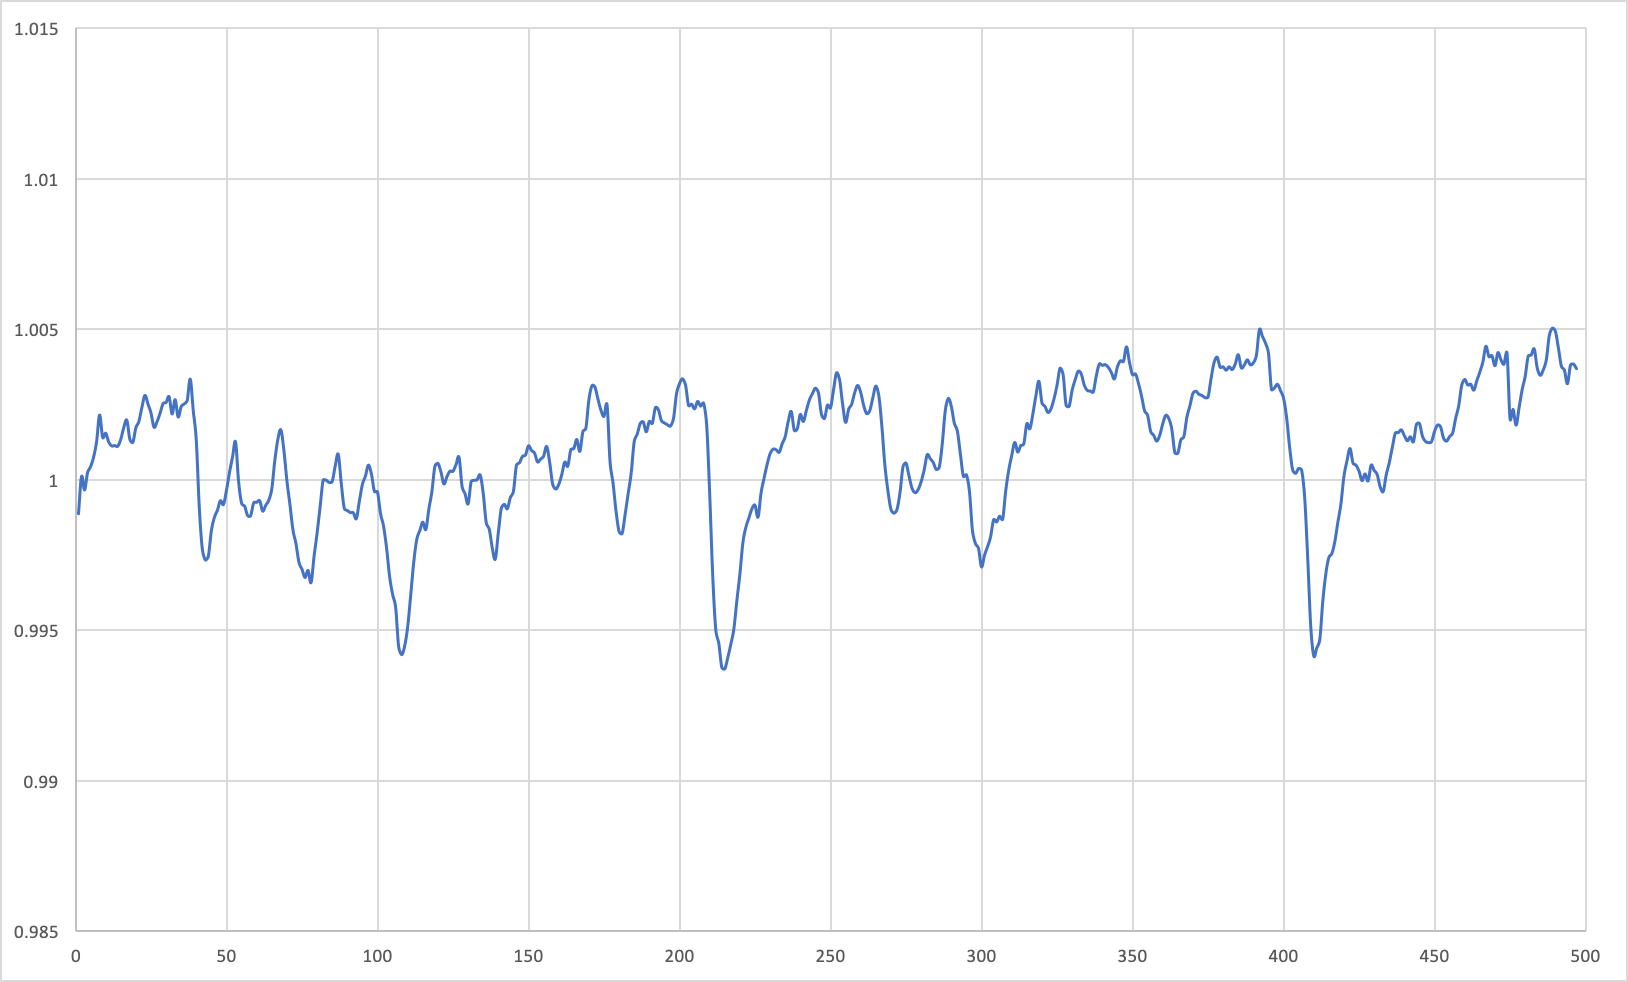
\includegraphics[width=1.0\textwidth]{Controls/10uF.png}
  \caption{\label{fig:10uF} LSM9DS1 accelerometer with $10\mu F$}
\end{figure}

\begin{table}[H]
\caption{\label{tab:99nF} LSM9DS1 Z-Axis Acceleration Statistics ($C=99nF$)}
\centering
\begin{tabular}{l|c}
\hline\hline
\textbf{Statistic}      & \textbf{Value}            \\\hline
Mean                    & $0.99862$                 \\\hline
Median                  & $0.99799$                 \\\hline
Mode  	                & $0.99814$                 \\\hline
Sample Variance         & $7.87\times10^{\minus6}$  \\\hline
Standard Deviation      & $2.81\times10^{\minus3}$  \\\hline
Standard Error  	    & $1.26\times10^{\minus4}$  \\\hline
Minimum                 & $0.99137$                 \\\hline
Maximum                 & $1.00466$                 \\\hline
\end{tabular}
\end{table}

\begin{figure}[ht]
  \centering
  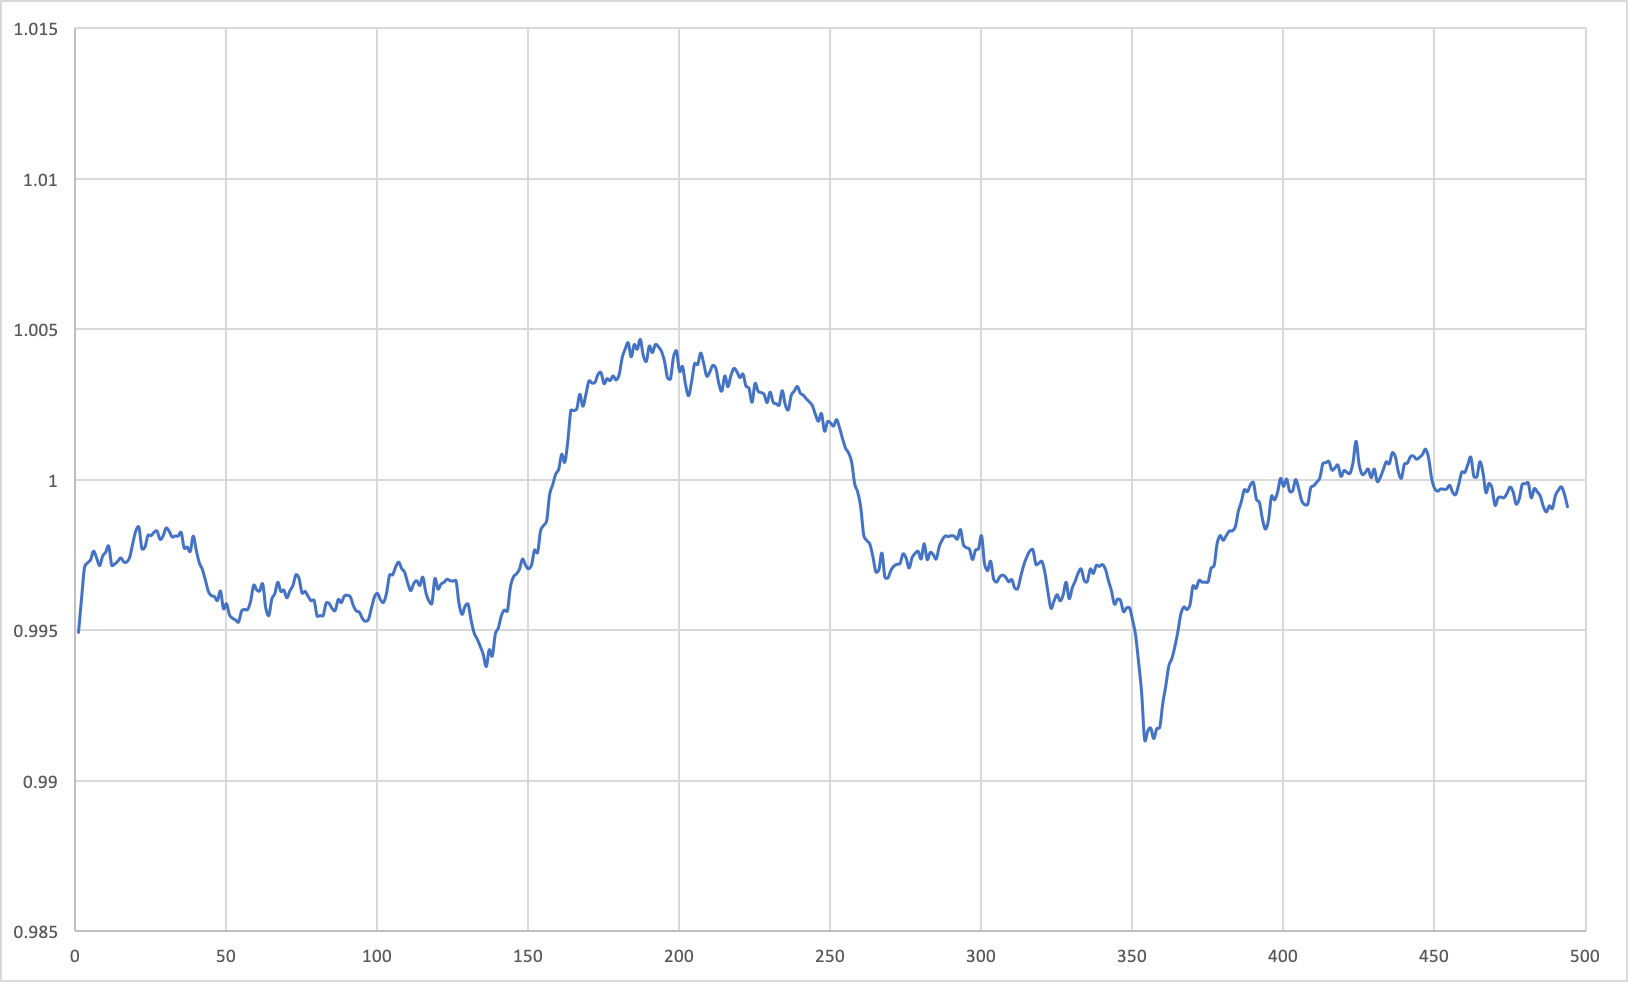
\includegraphics[width=1.0\textwidth]{Controls/99nF.png}
  \caption{\label{fig:99nF} LSM6DS3 accelerometer with $99nF$}
\end{figure}


As can be observed by the data collected and the statistics performed, the sensor's output displayed noise that was propagated down from the power line. When the sensor had no capacitor placed to clean up and smooth the signal, the output had the highest amount of fluctuation [Fig. ~\ref{fig:no_cap}] and a sample variance of $2.91\times10^{\minus5}$.

When a $10\mu F$ capacitor was put in place, the fluctuations diminished significantly as can be seen in [Fig. ~\ref{fig:10uF}], however a cyclic disturbance was observed at the $3kHz$ frequency once the sensor was placed under the oscilloscope, further investigation is required to better determine how to eliminate the noise from this frequency. Nonetheless, the mean, median, and mode are all very close to the true value of 1g corresponding to the acceleration experienced by the IMU while resting on the table. In addition, the sample variance dropped to $4.94\times10^{\minus6}$, an order of magnitude less compared to the case where to capacitor was placed.

Lastly, a $99nF$ capacitor was placed and data was collected and analyzed. Fluctuations in the readings were present, however such fluctuations were less than the case with no capacitor and had sudden sharp changes in readings. These results had led the design to incorporate a $10\mu F$ across the sensors' array [Fig. ~\ref{fig:rpi_imu_setup}] to shunt noise and get more reliable data readings.

\begin{figure}[ht]
  \centering
  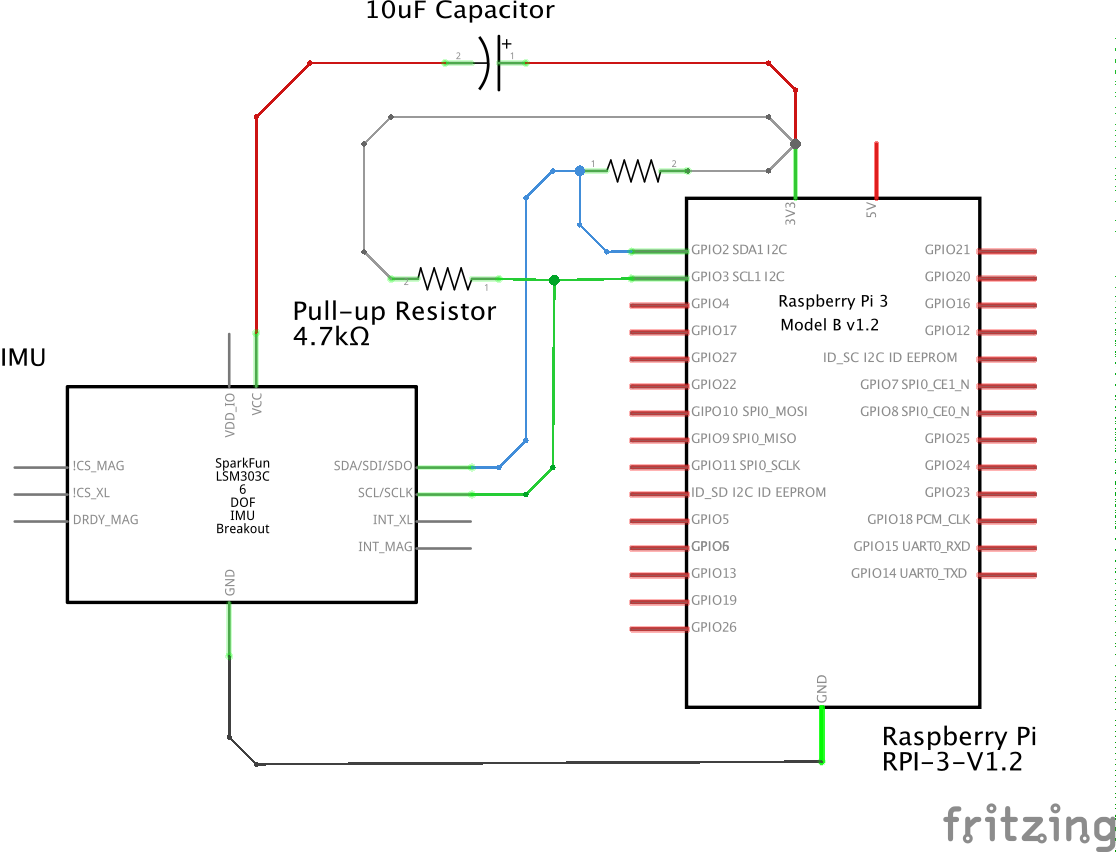
\includegraphics[width=0.8\textwidth]{Controls/rpi_imu_setup_schem.png}
  \caption{\label{fig:rpi_imu_setup} Sample setup }
\end{figure}

% ---------------------------------------------------------

\subsubsection{Temperature Sensor}

\indent\indent To validate the temperature sensor choice, a test comparing the readings of the TMP006 sensor against the temperature readings of a mercury thermometer readings in boiling water was carried on. Given that the TMP006 is a non-invasisve thermometer, the sensor was placed approximately a foot away from a pot of boiling water and data acquisition ran for 400 seconds, or approximately 7 minutes. The output of the sensor consisted of 4 averaged readings at a 16bit resolution at a frequency of $f_s=0.25$, or 1 reading per 4 seconds. The TMP006 readings tracked the mercury thermometer readings closely as was judged by eye measurements, however sudden spikes would occur at infrequent times.
After the data was acquired and analyzed, it was determined that a signal smoothing function needs to be implemented. The choice was to implement an exponential moving average (EMA) technique to smooth the data acquired, this is because the exponential moving average gives a higher weighting to recent prices compared to a simple moving average (SMA), which assigns equal weighting to all values. The EMA is defined mathematically in [Eq. ~\ref{eq:EMA}] below,

\begin{equation}
    S_t=
    \left\{ \begin{array}{ll}
        Y_0                             &   t = 0   \\
        \alpha T_t + (1-\alpha)S_{t-1}  &   t > 0   
    \end{array} \right.
    \label{eq:EMA}
\end{equation}

Where $0 < \alpha < 1$ is the smoothing factor, $Y_t$ is the sampled data at time $t$, and $S_t$ is the smoothed data at time $t$. One must take care of choosing an appropriate smoothing factor, if $\alpha$ is set to a high value, then the smoothed data is very responsive to recent changes and smoothing effects are minimal, whereas if $\alpha$ is set to an adequately low number then the smoothed data is not very responsive to recent changes. However, if $\alpha$ is set to a very low number, then the data is not responsive to recent changes and the smoothed data is not representative of the data collected. The one variable statistical analysis that was performed on both the raw and smoothed data is presented in [Table ~\ref{tab:raw_signal}] and [Table ~\ref{tab:ema_signal}], respectively,

\begin{table}[H]
\caption{\label{tab:raw_signal} TMP006 Raw Temperature Readings Statistics}
\centering
\begin{tabular}{l|c}
\hline\hline
\textbf{Statistic}      & \textbf{Value}            \\\hline
Mean                    & $106.098$                 \\\hline
Median                  & $106.425$                 \\\hline
Mode  	                & $102.200$                 \\\hline
Sample Variance         & $28.8907$                 \\\hline
Standard Deviation      & $5.37500$                 \\\hline
Standard Error  	    & $0.53750$                 \\\hline
Minimum                 & $96.0100$                 \\\hline
Maximum                 & $119.730$                 \\\hline
\end{tabular}
\end{table}

\begin{table}[H]
\caption{\label{tab:ema_signal} TMP006 Smoothed Temperature Readings Statistics}
\centering
\begin{tabular}{l|c}
\hline\hline
\textbf{Statistic}      & \textbf{Value}            \\\hline
Mean                    & $104.835$                 \\\hline
Median                  & $107.119$                 \\\hline
Mode  	                &   \#N/A                   \\\hline
Sample Variance         & $21.3482$                 \\\hline
Standard Deviation      & $4.62041$                 \\\hline
Standard Error  	    & $0.46437$                 \\\hline
Minimum                 & $97.3200$                 \\\hline
Maximum                 & $110.690$                 \\\hline
\end{tabular}
\end{table}

\begin{figure}[ht]
  \centering
  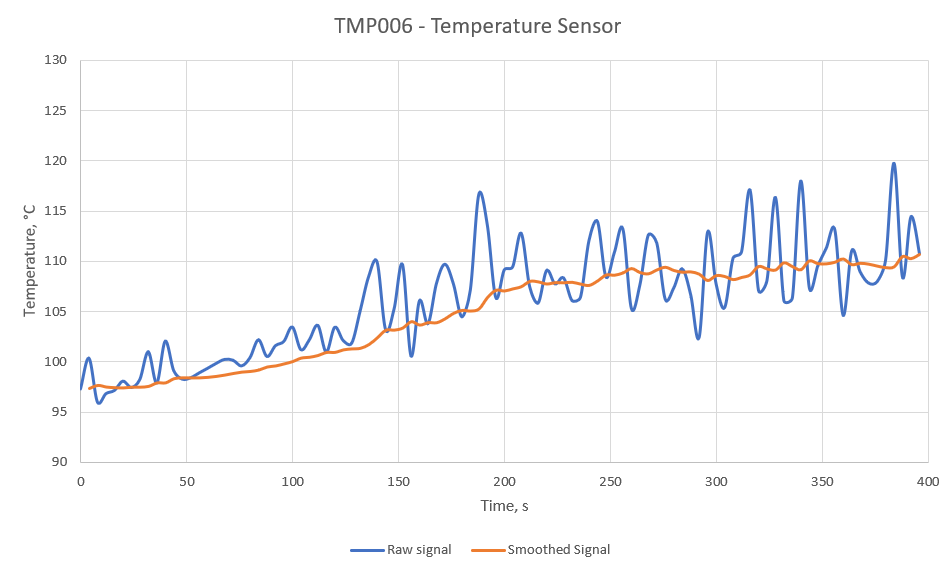
\includegraphics[width=1.0\textwidth]{Controls/tmp006_signal.PNG}
  \caption{\label{fig:raw_vs_ema} Raw vs. EMA Smoothed TMP006 Readings}
\end{figure}

As can be observed from the graphs and data, the EMA filter help reduce and attenuate the sudden sharp spikes in readings and in turn return a more reliable data readings that better mimicked the data readings of the mercury thermometer. However, after multiple tests, it was observed that the TMP006 non-invasive temperature readings were greatly affected by the color and gloss of the surface it was pointed it. For instance, if the surface was very bright in color and/or had a glossy finish, the readings would fluctuate and spike. Whereas if the surface had a dark color and/or a matte finish, the readings were very accurate and had very minimal spikes.

It must be noted that reading accuracy can be sacrificed for a faster sampling rate, for instance, an 8bit resolution reading would have a sampling frequency of $f_s=1.00$, or 1 sample per second. Nonetheless, 16bit resolution readings was chosen since temperature readings are not critical for the system's operation in real-time.

% ---------------------------------------------------------

\subsubsection{Motor Controller}

\indent\indent The VEX Victor BB High-Voltage Controller was chosen as the motor controller of choice since it was recommended by the manufacturer. Initial attempts to use the motor controller resulted in failure to establish communication with the controller. After multiple failed attempts, the team reached out to VEX Robotics support engineers, who in turn directed the team to get in contact with CTR Electronics sales engineers given that the firmware running the motor controller is developed by them. After being instructed that the PWM signal had to have a duty cycle length of $1.5ms - 2.0ms$ and the code adjusted accordingly, the the motor controller was fully functional and operational.

% ---------------------------------------------------------

\subsubsection{Brakes Actuator}

\indent\indent The choice of actuator was governed by the amount of force it needed to apply to the master cylinder to engage the brakes. After diligent research, the an optical feedback linear actuator with a 6 inch stroke length and $400lbs$ of force from Firgelli was picked due to having ample stroke length, force, internal limit switches, and an optical feedback of extension value. The team members attempted to control the actuator using an H-Bridge, however due to the availability of a more sophisticated linear actuator controller board provided by Firgelli, the team opted to use the linear actuator controller board which is controlled via PWM. In accordance to the documentation, the PWM signal had to be at a frequency of $1kHz$, where the percent duty cycle load corresponded to the percent extension value of the actuator. In other words, if the PWM had a duty cycle load of 0\% then the actuator is fully retracted, 50\% is equivalent to the actuator being extended halfway its full length, and 100\% is equivalent to the actuator being fully extended. After incorporating the code written by the MAE team into the CS team's codebase, the actuator was tested and proved to work as intended.

% ---------------------------------------------------------

\subsubsection{Radio Trasnmitter/Receiver}

\indent\indent The radio transmitter/receiver modules were chosen by the CS team. Their choice fell on Digi International XBee® SX RF Modems. The decision to choose said radio module was due to it's relatively affordable price compared to other radios in the same features range. In addition, the module has a high transmission range of 65 miles, and is capable of sending/receiving messages at a frequency of $f=10Hz$, or 1 message per 0.1 seconds. After setting up the radios, the CS team was able to demonstrate their abilities by sending and receiving data while being situated in two different buildings.